\chapter[Proposta de Solução]{Proposta de Solução}\label{cap2}

A proposta de solução deste trabalho é um produto interdisciplinar na união dos cinco cursos de engenharia presentes no campus UnB - Gama, com o intuido de resolver os problemas apresentados no capítulo anterior. A proposta inicial de solução é desenvolvimento de um alimentador automático, com capacidade de regarga de bateria via energia solar e de armazenamento de ração para um período rasoável de autonomia. A implementação desta proposta envolve diversas áreas de conhecimento e estará melhor detalhada nas seções seguintes.
A organização da apresentação da solução está baseada em sub-sistemas que integrados resultarão na solução como um todo.

\section{Requisistos do Sistema}

Está sessnao lista os requisitos de projeto, tanto do cliente quanto dos projetistas.

\subsection{Requisitos Eletrônicos}

\begin{itemize}
  \item O sistema deve ser capaz de avaliar o nível de bateria que alimentam os dispositivos de cada tanque;
 \item Características da água como a temperatura, o pH, a condutividade, a turbidez e o O2 dissolvidos devem ser avaliados pelos sensores presentes no tanque;
\item Devem ser avaliados o nível de ração no primeiro reservatório e a quantidade de ração no segundo reservatório;
\item O microcontrolador deve ser responsável por acionar os motores presentes nos tanques de acordo com a taxa temporal e períodos necessários para cada um;
\item Devem ser comportados até 30 tanques dentro da rede sem fio;
\item As informações sobre taxas de tempo e quantidade de ração a ser despejada devem ser enviadas da base para os dispositivos nos tanques;
\item As informações dos sensores presentes nos tanques devem ser enviadas para a base pela rede sem fio quando solicitadas por elas.
\end{itemize}

\subsection{Requisitos Estruturais}

O requisitos estruturais são relacionados ao volume, massa e disposição dos elementos na estrutura, além de suas funcionalidades:

\begin{itemize}
  \item Armazenar 300kg de ração;
  \item Gerar sustentação hidroestática para toda a massa do sistema estimada em 400kg, além das carga eventual do tratador e saco de ração no momento do reabastecimento;
  \item Minimizar efeitos térmicos da alta incidência solar da área de atuação do sistemam para preservar a qualidade da ração;
  \item Transportar a ração do Armazenador para os tanques rede;
  \item Possuir a maior estabilidade possível em relação ao tratador nos momentos de reabastecimento e em rajadas de vento média da região;
  \item Abrigar os subsistemas embarcados;
  \item Isolar a ração e os subsistemas embarcados da umidade;
\end{itemize}

\subsection{Requisitos Energéticos}
\begin{itemize}
  \item O local deve ter insolação suficiente para que a placa fotovoltaica seja capaz de fornecer energia ao sistema.
\item A bateria deve armazenar energia elétrica para ser capaz de alimentar todo o sistema mesmo quando não houver sol.
\item O motor deve possuir potência suficiente para fazer o fuso girar e levar ração até o reservatório inferior.
\item A ração deve ser arrastada pelo fuso e cair diretamente no reservatório inferior, não se dispersando.
\end{itemize}
\subsection{Requisitos do sistema de controle}
O requisitos sistema de controle são relacionados à interface do usuário e parametros de configuração

\begin{itemize}
  \item O sistema deve ser capaz de modificar a configuração do sistema embarcado do alimentador
  \item O sistema deve gerenciar níveis de acesso, ou seja, alguns usuário não teram acesso a todas as funcionalidades
  \item O sistema deve ser de fácil utilização e interpretação uma vez que o conhecimento técnico do usuários é baixo
  \item O sistem deve funcionar de forma local uma vez que o ambiente de produção não possui acesso de internet confiavel, ou seja, pode não haver acesso à internet
\end{itemize}

\section{Limitações}
Está sessão aborda as limitações do projeto, isto é, o que o a solução não resolverá ou não poderá desenvolver
devido a escolhas ou limitações.

\subsection{Limitações Eletrônicas}
A escolha de todos os componentes eletrônicos utilizados no alimentador estão, basicamente, condicionados ao consumo energético, uma vez que o sistema depende da alimentação de uma bateria que é recarregada esporadicamente durante a atividade solar.

Um fator que poderia ser limitante é a dimensão física dos componentes, que deverão ser alojados dentro de uma carcaça que não ocupe uma dimensão considerável do alimentador. Como a capacidade do tanque de ração está prevista para 300 kg, o volume do ocupado pela parte eletrônica não deve ser preocupante, em vista da relativa baixa quantidade de componentes e sensores requeridos para a atividade do alimentador.

Devido ao produto ser concebido para estar exposto a um ambiente bastante úmido e suscetível à tempestades e movimentação intensa da água, será utilizada uma carcaça que guarda todos os componentes e que deverá ser mantida totalmente selada. Por conta de alguns componentes que aquecem acima do comum, como os drivers do motor, não havendo disponível a circulação de ar para dissipar o calor gerado e refrigerar o circuito integrado , devendo ser dimensionado para operar frio.

\subsection{Limitações Estrutuais}
Componentes como o transportador de alimentos só terá sua efetividade comprovada a partir de testes exaustivos feitos com diferentes granulometrias de ração.

Na parte de isolamento térmico não foi encontrados dados técnicos sobre o produto, apenas dados comerciais, dificultando assim uma comparação mais precisa de soluções possíveis.

\subsection{Limitações de Software}

Uma vez que o ambiende de produção do projeto como um todo é de dificil acesso à conexão de internet, o projeto tem como principal objetivo o funcionamento do sistema e controle de forma local. Após o funcionamento de forma local há a intenção de se trabalhar um forma de sincronização online. Porém este ultimo não faz parte do escopo principal.

\section{Visão geral da solução}

De acordo com o que foi apresentado no termo de abertura do projeto, a solução proposta envolve diversos módulos funcionais, são eles: o alimentador, a base, e o sistema de controle SCADA. A partir de uma visão de alto nível do projeto, como a apresentada na Figura \ref{diagrama}, é possível observar de maneira clara os módulos que deverão se comunicar para garantir o funcionamento do sistema como um todo.

\begin{figure}[H]
 \centering
   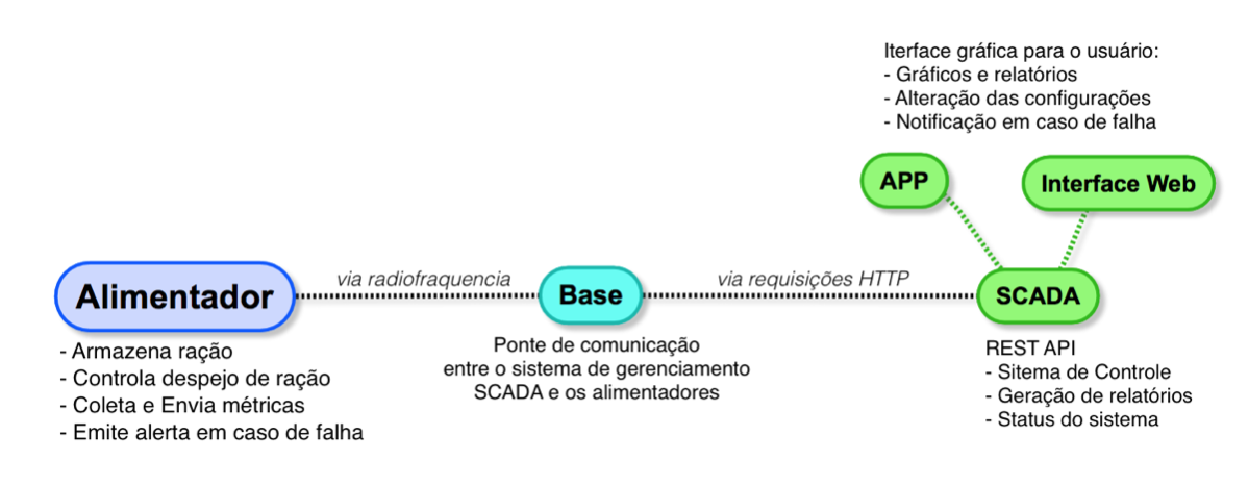
\includegraphics[keepaspectratio=true,scale=0.8]{figuras/digrama_geral.eps}
 \caption{Arquitetura geral da solução}
 \label{diagrama}
\end{figure}

Para garantir que a solução seja responsável, do ponto de vista de situações críticas, como a falha na comunicação entre os alimentadores e base, os alimentadores possuem autonomia de funcionamento, isto é, são capazes de operar independentemente. Tendo por base a configuração presente no equipamento.

Uma vez que o alimentador estará presente no tanque de peixe e este, por sua vez, pode ficar distante da margem, pareceu-se conveniente a utilização de uma via de comunicação de grande alcance(radiofrequência) para se comunicar com um aparelho base responsável por receber informações dos alimentadores e envia-las para o sistema de controle SCADA através de uma rede local.

O sistema SCADA consiste de uma API REST responsável por receber e armazenar os dados dos alimentadores e deve disponibilizar de forma estrutura para os gestores da piscicultura através de uma interface gráfica web e mobile.
